\documentclass[11pt]{article}
%\geometry{landscape}                % Activate for for rotated page geometry
%\usepackage[parfill]{parskip}    % Activate to begin paragraphs with an empty line rather than an indent
\usepackage{graphicx}
\usepackage{epstopdf}
\usepackage{enumitem}
\usepackage{subcaption}
\usepackage{csquotes}
\def\myhyphen{{\hbox{-}}}

\title{Cosmic-ray reconstruction efficiency measurement using an external cosmic-ray counter}
\author{Stefano Roberto Soleti}
\date{\today}                                           % Activate to display a given date or no date

\begin{document}
\maketitle
\section*{Questions asked during the Collaboration Meeting}
\begin{description}[style=nextline]
  \item[Elena - Do you use an angular cuts to select your events?]
  It is possible to apply an angular cut to our sample in order to increase the purity. However, the increase in the purity applying a cut of 2$^{\circ}$ on the difference between the extrapolated angles and the reconstructed ones ($\Delta\theta$ and $\Delta\phi$) is less than 0.1\% and it has been considered negligible. The histograms of the angular differences and the results of the cut have been added to the Appendix A of the last version of the internal note.
  \item[E - Are you accounting for decays between in the TPC?]
  No, because when we started this analysis the efficiency was not high enough to consider this effect relevant. However, with the last version of the analysis and an overall efficiency of 96.1\%, the effect of muons triggering the MuCS and decaying or being captured before reaching the TPC must be taken into account. The fraction of this kind of events is $(1.0 \pm 0.1)$\% and the value of the efficiency has been corrected accordingly. A detailed study of this effect has been included in section 5.1 of the last version of the internal note.
  \item[Leon - If you make an angular cut, then the scatter plot of points of the MuCS will look nicer?]
  Yes, the effect of the angular cut would be to remove the events with a large scattering of the cosmic muon. Figure \ref{fig:alignment} shows the extrapolated points for the upstream configuration before (\ref{fig:upstream}) and after (\ref{fig:upstream_after}) an angular cut of 5$^{\circ}$ on $\Delta\theta$ and $\Delta\phi$. However, the point of that plot was to show that the majority of the MuCS-tagged tracks can be extrapolated back to the height of the panels.
  \begin{figure}[htbp]
    \begin{subfigure}{0.5\textwidth}
      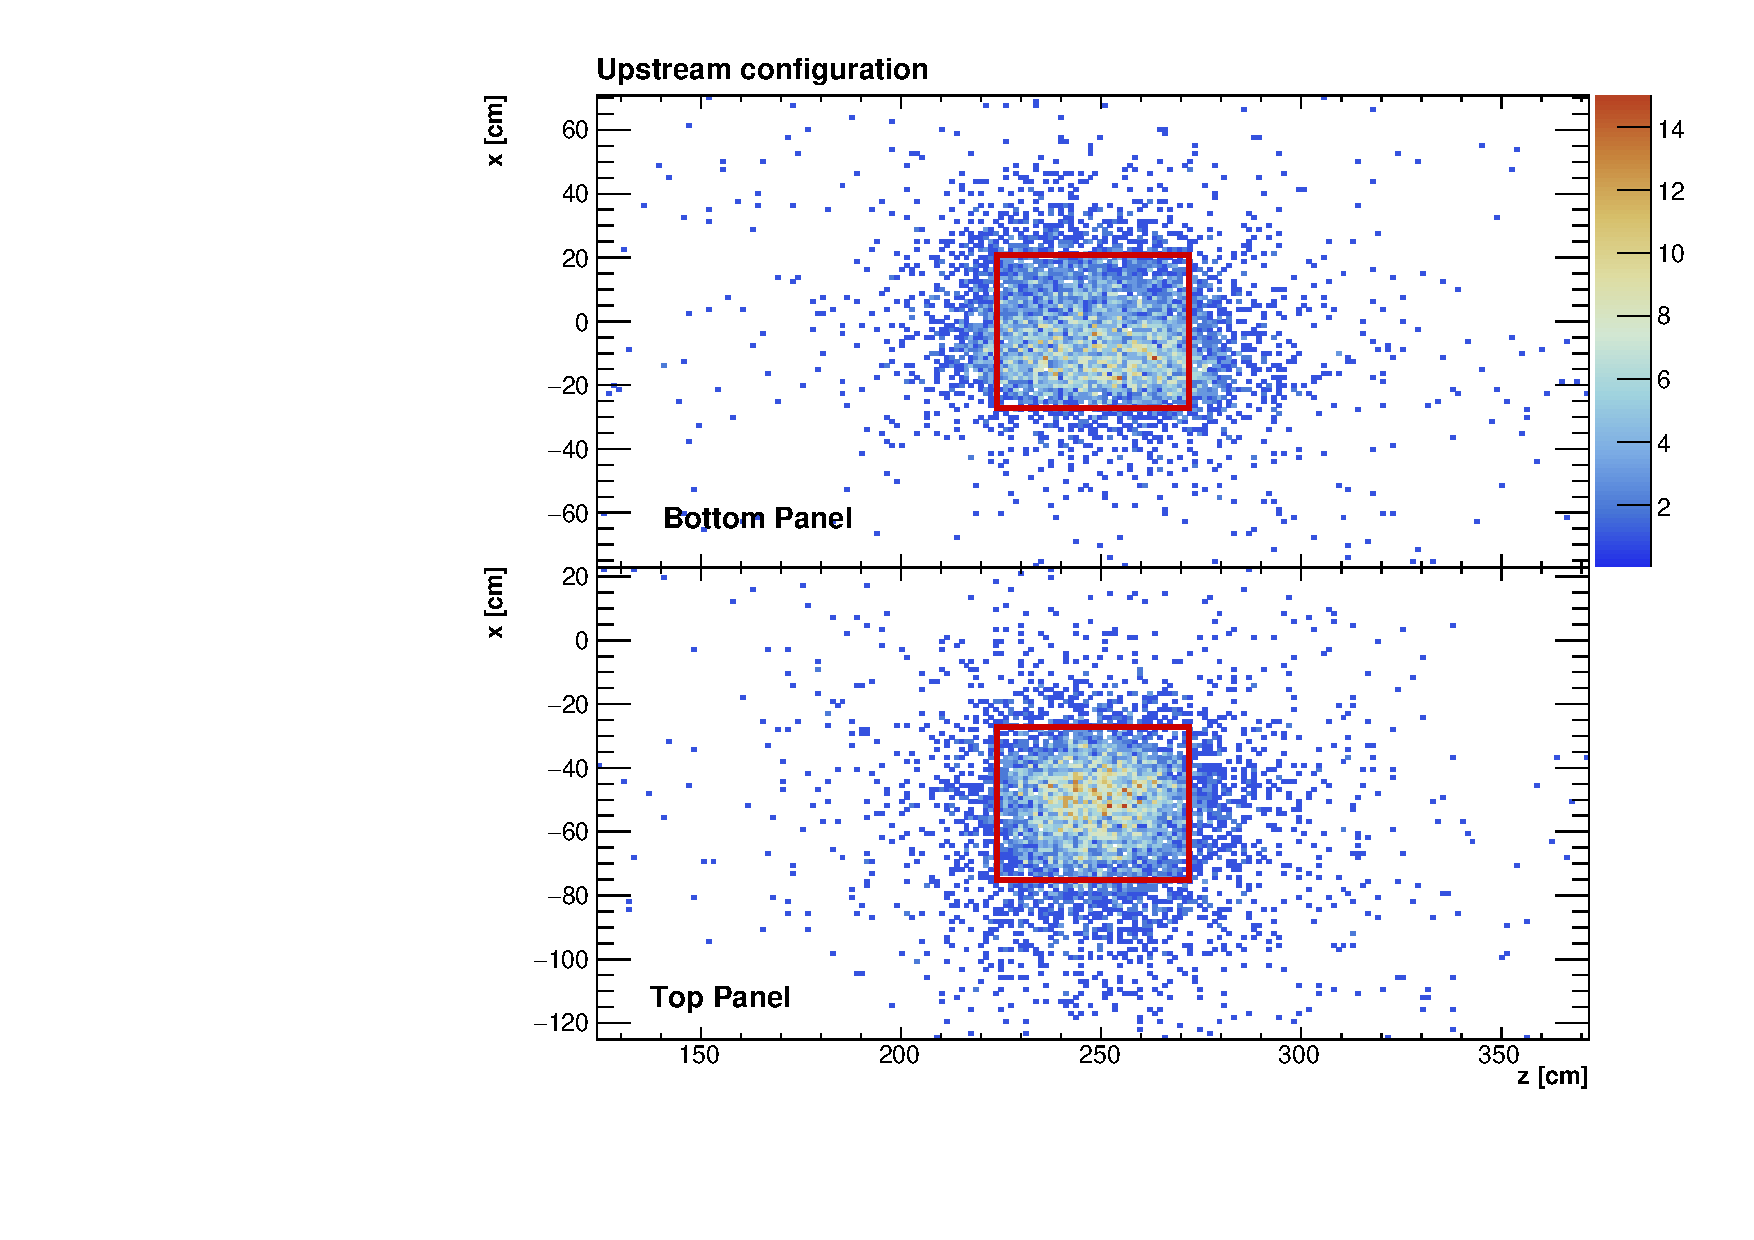
\includegraphics[width=\linewidth]{../figures/upstream.pdf}
      \caption{Upstream - before angular cut} \label{fig:upstream}
    \end{subfigure}
    \begin{subfigure}{0.5\textwidth}
      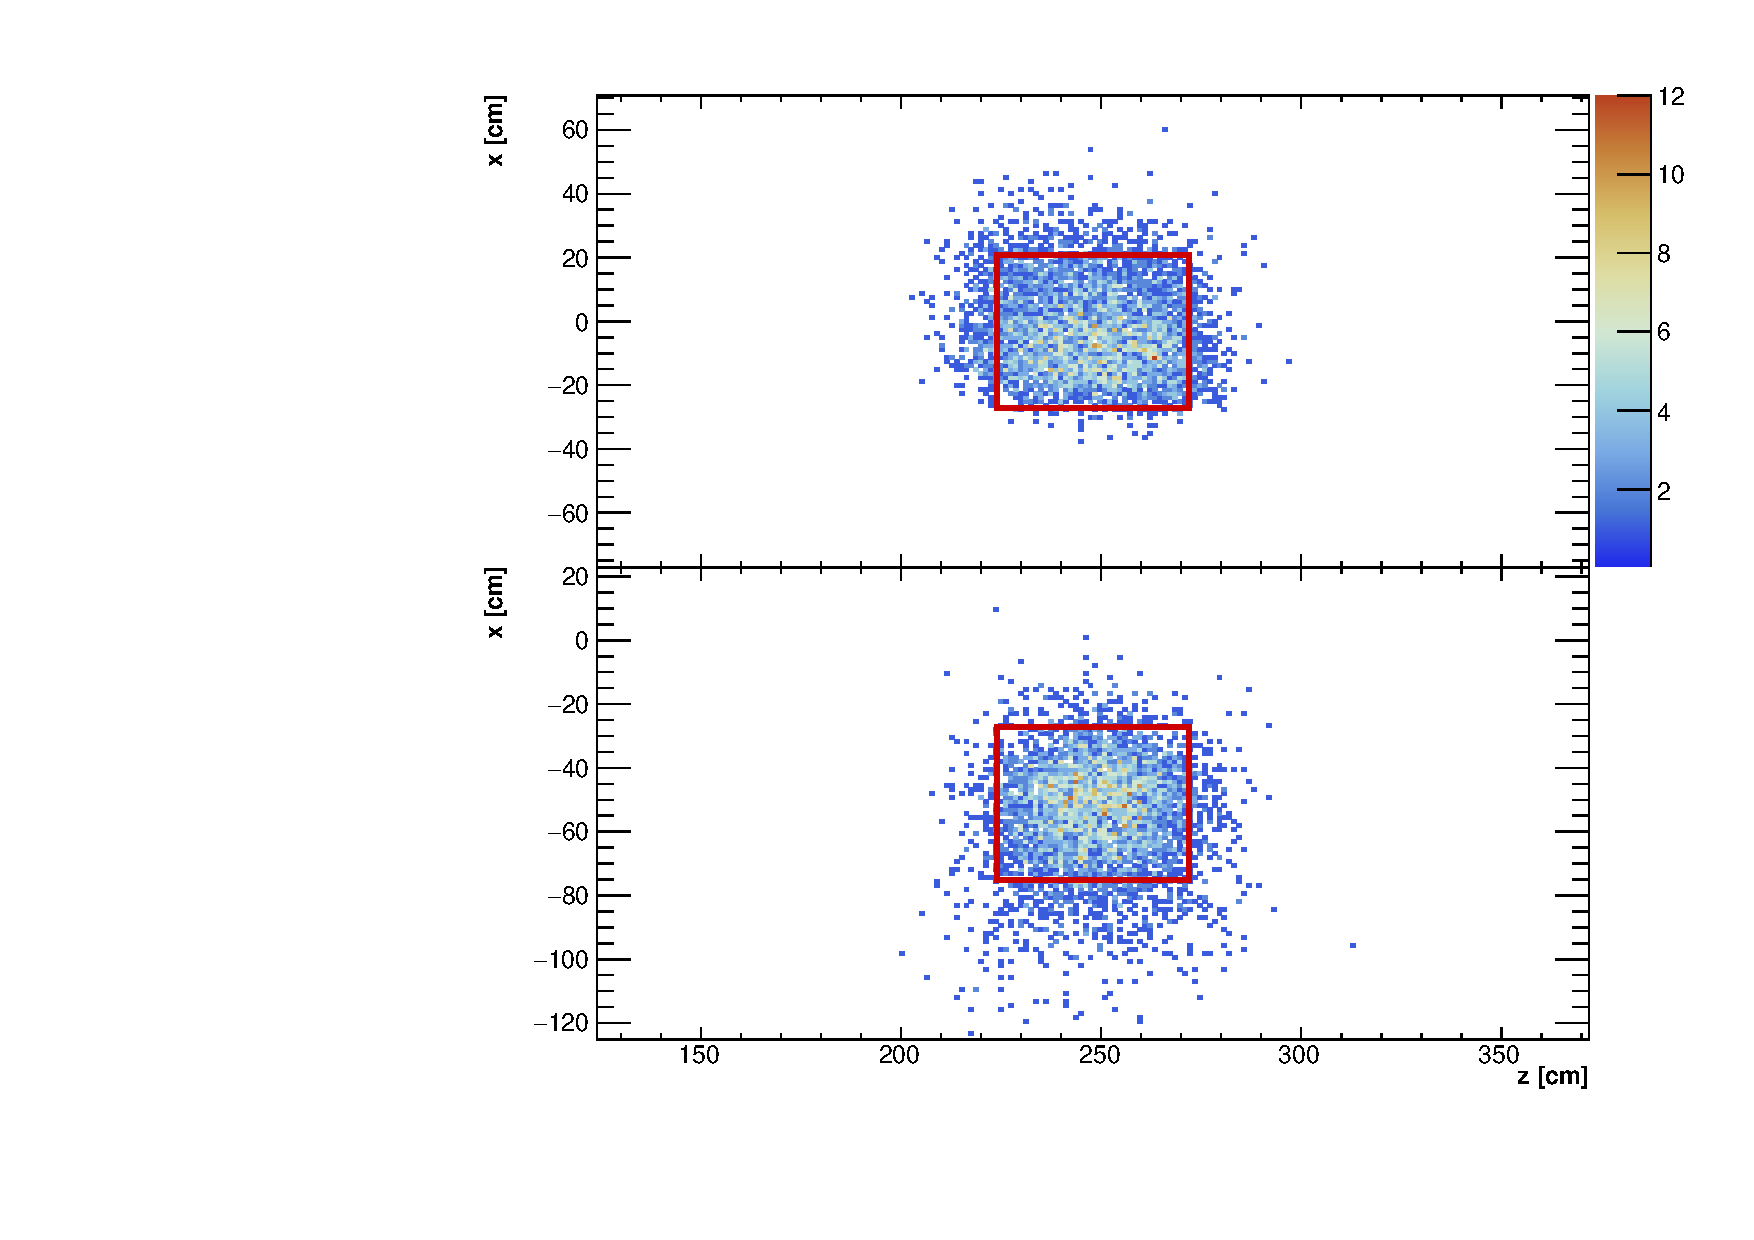
\includegraphics[width=\linewidth]{../figures/upstream_after.pdf}
      \caption{Upstream - after angular cut} \label{fig:upstream_after}
    \end{subfigure}

    \caption{Extrapolated points of the MuCS-tagged tracks at the height of top and bottom panels for the upstream configuration before and after an angular cut of 5$^{\circ}$ on $\Delta_{\theta}$ and $\Delta_{\phi}$.} \label{fig:alignment}
  \end{figure}
  \item[Mike K - How do you reconcile 96.1\% reconstruction efficiency with the few percent efficiency quoted by Tim Bolton?]
  Our efficiency and the one quoted by Tim cannot be compared directly. In our case, every event has a MuCS cosmic ray and we measure the fraction of those events with a reconstructed track, while Tim's 6\% includes CC-inclusive event selection.
\end{description}

%\subsection{}

\section*{EB questions}
\begin{description}[style=nextline]

\item[Andrew - line 95 - From figure 2, I see that not all MuCS muons pass through the TPC. Can you confirm that this has no effect on the calculated efficiencies? I'd guess that the requirement of both a PMT and MuCS signal in the trigger ensures that we only count the muons that pass through both the MuCS and TPC. It might be worth adding a sentence about this somewhere in the internal note.]
Actually, the fraction of events hitting the MuCS and missing the TPC is, according to the MuCS Monte Carlo, 0.3\%. In order to remove these events from our sample, we check if the extrapolated trajectory in the TPC is longer 20 cm. I added a sentence in section 5 explaining this.


\item[A - line 133 - I'd insert a new section header 'Monte Carlo simulation' at this point. Am I right in saying that the MuCS system isn't explicitly included in the G4 simulation? You should probably say this in the internal note.]
Correct. I added a sentence to clarify this.

\item[A - line 147/148 - I'm confused about how you filter MC events (sorry!). Lines 147/48 imply that you discard Monte Carlo muons outside the angular acceptance of the MuCS. However, in order to calculate the quantity P (i.e. purity), I think you'd need to use a MC sample covering the full range of angles. Could you clarify? I have a similar question about lines 189/90. When you calculate P and A from the MC, do you require that the MC muons pass through the known locations of the MuCS panels? I think perhaps not, given the statement in 167/68 about an independent MC sample. It might help to add some extra text to the note about this.]
I am sorry, probably the text wasn't clear. I rewrote sec. 5 in the last version of the internal note: long story short, we have two Monte Carlo samples. One is the MCC7 cosmic-ray sample, with cosmic rays generated all over the TPC, and one is the MuCS Monte Carlo, used to measure the angular distributions and the P, A parameters. The MuCS Monte Carlo is generated as explained in 167-170. So, to answer your question, when we measure P and A we require the MC muons to pass through the locations of the panels.

\item[A - Figure 5 (around line 162) - Figure 5 looks nice! Could you label the upper and lower panels 'Top' and 'Bottom'? Also, you should probably write the labels 'Upstream', 'Center' and 'Downstream' onto the plots themselves (so that these plots will make sense when shown separately in talks). The axis labels 'x' and 'z' are also a bit too small on these plots.]
Right, I added the labels.

\item[A - Figure 7 (around line 208) - Thanks very much for adding the data points to figure 7 (something I requested). I think the data look good. The fact that both the data and MC reconstruction efficiencies have a flat dependence on $d_{\mathrm{max}}$ indicates that the quantity P/A (in particular the acceptance) is well-modeled by the MC, which is good. By the way, do you apply the same P/A correction to each of the different MuCS configurations?]
Yes, the P/A correction is applied to the merged sample, so same value for the three configurations.

\item[A - around line 208 - In a previous thread, Vassili suggested making a plot of the $d$ variable. I think a data/MC comparison of this variable might be a good plot for the internal note.]
We agree this is a useful plot. Figure \ref{fig:dist} shows the distribution of the $d$ variable for data and Monte Carlo. As you can see, there are some small discrepancies, but our cut is in the region where the number of events is low and the differences between data and Monte Carlo are negligibile.

\begin{figure}[htbp]
\begin{center}
  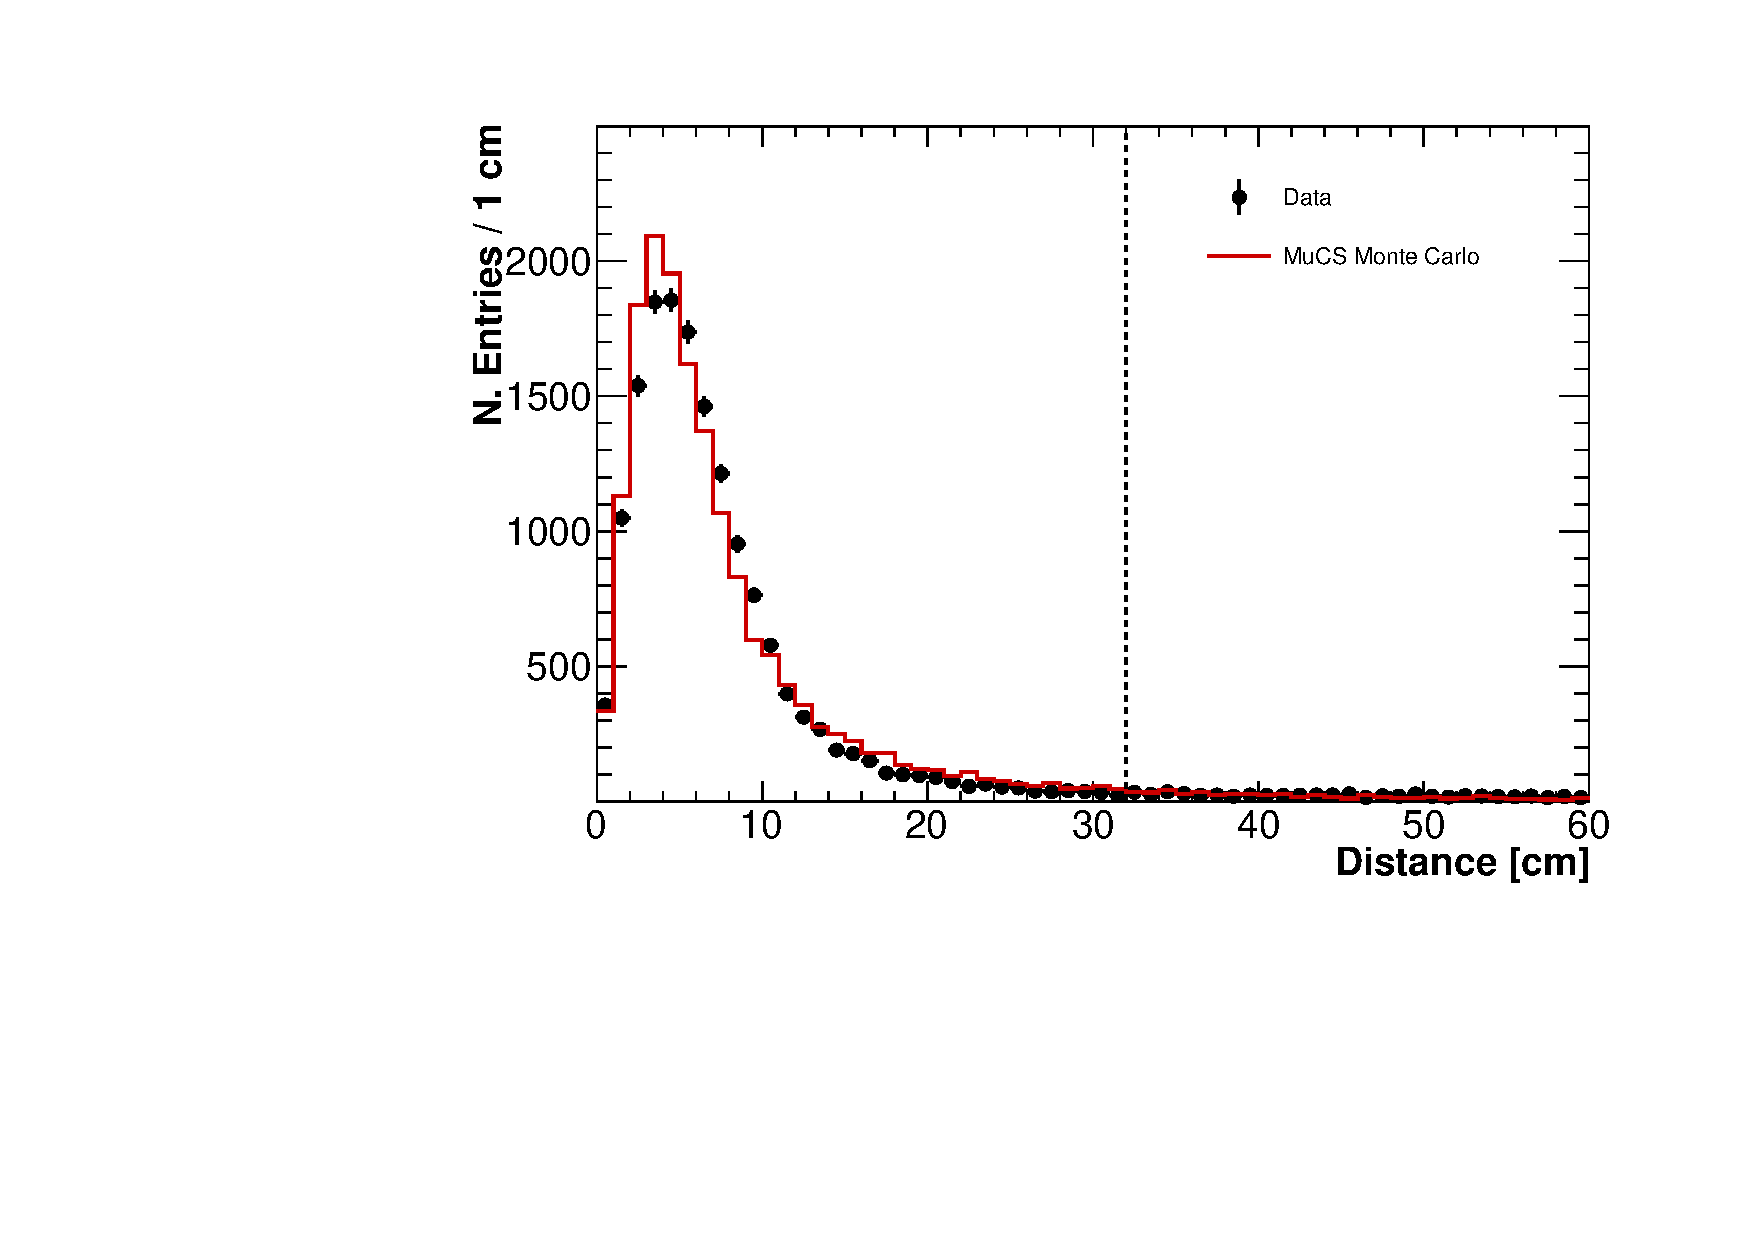
\includegraphics[width=0.7\linewidth]{../figures/dist.pdf}
  \caption{Distribution of the distance between the extrapolated starting point and the reconstructed track startin point for data (black points) and Monte Carlo (solid red line).} \label{fig:dist}
\end{center}
\end{figure}

\item[A - around line 220 - I wonder if, at this point, you could quote the calculated values of $\epsilon_{\mathrm{MC}}$ and $\epsilon_{\mathrm{data}}$ in the text with their statistical errors (i.e. 96.1\% and 96.3\%)? (It might be nice to do this before the discussion of systematics). Could you also include a table showing the separate $\epsilon_{\mathrm{MC}}$ and $\epsilon_{\mathrm{data}}$ values for each of the three different MuCS configurations? I'm assuming there are three different values of $\epsilon_{\mathrm{MC}}$, but I might be mistaken.]
Right, I'll add a table with the $\epsilon_{\mathrm{data}}$ and $\epsilon_{\mathrm{MuCS-MC}}$ values for each configuration. The value of $\epsilon_{\mathrm{MC}}$ is only one, because it is obtained generating cosmic rays all over the TPC, but, yes, there are three different values of $\epsilon_{\mathrm{MuCS-MC}}$.

\item[A - Figure 8 (line 219) - The 3D (or 4D?) plots in figure 8 look cool - but I wonder if they're too hard to absorb? Also, only the outer edges of these plots can ever be visible. I think the 1D and 2D plots in figures 13 and 14 do a good job of getting the message across.]

We agree that the 4D plots in figure 8 are not good to show the real values. However, we think they might be useful to show our approach, that is to have a reconstruction efficiency as a function of three different parameters, that we can reduce to two or one projecting the original 4D distribution on a plane or on an axis.

\item[A - line 221 - I'd insert a new section header 'Systematic Uncertainties' here.]
Done.

\item[A - line 252 - You should quote the overall systematic error resulting from non-uniformities in the text at this point (it looks like the number is 1.1\%?).  This seems like it's probably an over-estimate, since: (1) detector uniformities are included in the simulation to some extent, (2) figure 9 doesn't suggest that the systematic error would be so large. Can you clarify in the text how you get to 1.1\% - I guess the best MuCS efficiency is 1.1\% higher than the average efficiency? I'm not suggesting that you change the method - just clarify in the text.]
Yes, that 1.1\% means that the best configuration has an overall efficiency 1.1\% higher than the average one, I added a sentence to explain this. Regarding point (1), it is true that detector non-uniformities are included in the MC, but since we are considering a complete sample of cosmic rays, generated all over the TPC, their effect is negligible compared to our sample, where a consistent fraction of our cosmic rays go through a region with missing wires. For point (2), yes, the effect is only 1.5$\sigma$ but cannot be directly compared to the 1.1\%, since the former is a bin-by-bin significance histogram, while the latter is an overall difference.

\item[A - around line 273 - Is there a possible extra systematic associated with the calculation of the purity P? This quantity probably depends on the angular distributions of cosmic-ray muons being well-simulated. However, it's hard to imagine this being a large effect!]
The systematic associated to the P/A calculation has been quoted as 0.2\% and its evaluation is describe in the last version of the note: essentially. We also tried to remove events with reconstructed angles that differ more than $2^{\circ}$ from the extrapolated ones, but the increase in the purity is in the order of 0.1\% and it has been considered negligible. See Appendix A in the note for further info.

\item[A - Figure 13 (around line 277) - Are the MC errors in these figures stats-only? You should clarify this in the caption of figure 13. Also, I might change the y-axis titles from 'Efficiency' to 'Track reconstruction efficiency' in these plots.]
Right, I added a sentence in the caption. For the title, I will wait for other EB members to comment on the plot style, since we will also need to remove the "MicroBooNE in progress" labels before publishing the plots.

\item[Vassili - My main suggestion is that I would still like to see the distribution of the distances d between a TPC and a MuCS track. This quantity $d_{\mathrm{max}}$ defines the efficiency, since increasing the cutoff makes it more likely that a track will be found, thus increasing the apparent efficiency. Maybe Eq. 9 takes care of the issue, but the fact that $d_{\mathrm{max}}$ is chosen so that $P/A = 1$, effectively eliminating this factor, makes the whole approach seem a little like a slight-of-hand. I have no idea if this choice of $d_{\mathrm{max}}$ is sensible without seeing the $d$ distribution. It shouldn't be hard to make, since d is already calculated for every event.]
That's a good cross-check we didn't think about, thanks. You can see in figure \ref{fig:dist} that there are some small discrepancies between data and Monte Carlo, but around the region of our cut the difference is negligible and we think that our choice of $d_{\mathrm{max}}$ is therefore appropriate.

\item[V - Table 1: How where these positions determined? By surveying?]
Yes, we added a sentence to clarify it.

\item[V - ll. 218-218: I don't understand the statement that "The small dependence ... is due to the small discrepancies between the trend ..." at all. Could you rephrase it to clarify?]
We mean that, while the grey solid line is horizontal by construction (doesn't depend on $d_{\mathrm{max}}$), the grey dashed line is not, since $\epsilon^{\mathrm{data}}_{\mathrm{tag}}$ has a slightly different trend than $\epsilon^{\mathrm{MuCS\myhyphen MC}}_{\mathrm{tag}}$. We changed to sentence to:

\begin{displayquote}
  Using eq. (4), our MuCS Monte Carlo reconstruction efficiency $\epsilon_{\mathrm{MuCS\myhyphen MC}}$ will not depend, by construction, on the chosen value of $d_{\mathrm{max}}$. Since the $P/A$ correcting factor has been measured with a Monte Carlo simulation, the data reconstruction efficiency $\epsilon_{\mathrm{data}}$ will have a small dependance on $d_{\mathrm{max}}$ (see figure 7), because of the small difference between $\epsilon^{\mathrm{data}}_{\mathrm{tag}}$ and $\epsilon^{\mathrm{MuCS\myhyphen MC}}_{\mathrm{tag}}$.
\end{displayquote}

\item[V - l. 225: "having a minimal dependence ..." Where was this checked? (Sorry if I missed it.)]
We mean that, since the cosmic rays are generated all over the TPC and not in specific parts of detector as in the MuCS Monte Carlo, the dependence of the reconstruction efficiency on the position is minimal, because it's "averaged" on the entire volume.

\item[V - Fig. 7: Maybe this is a little outside the scope of this paper, but why is there a small difference between the reconstruction efficiencies in data and Monte Carlo? (Last two lines in the legend.) Do we understand this? Is it due to more noise in the data than was added in the MC?]
The difference between data and Monte Carlo is around 0.2\%. We think that, with a statistical error of 0.1\%, the two numbers can be considered in good agreement. However, a possible reason could be the absence of the MuCS panels volume in the GEANT4 stage of the Monte Carlo, which slightly increase the multiple Coulomb scattering of the muons in the data.

\item[V - l. 256: "significance is probably not the word usually used for something like this quantity. Maybe "normalized difference," or some other word? (This appears several more times below, so it would be a significant change.)]
We think that significance is the right word, because we are measuring if the discrepancy between two reconstruction efficiency values is significant or if it is within the statistical error.

\item[V - Fig. 10: The quantity plotted is not really dE/dx, although it could be related to it, when it's not noise. It's just an electronic signal. Maybe "collected charge" would be more appropriate.]
Right, we changed it to "collected charge".

\end{description}


\end{document}
